\documentclass[tikz,border=8pt]{standalone}

\usepackage{tikz}
\usetikzlibrary{positioning,arrows.meta}
\usepackage{xcolor}
\usepackage[T1]{fontenc}
\usepackage{lmodern}

\begin{document}
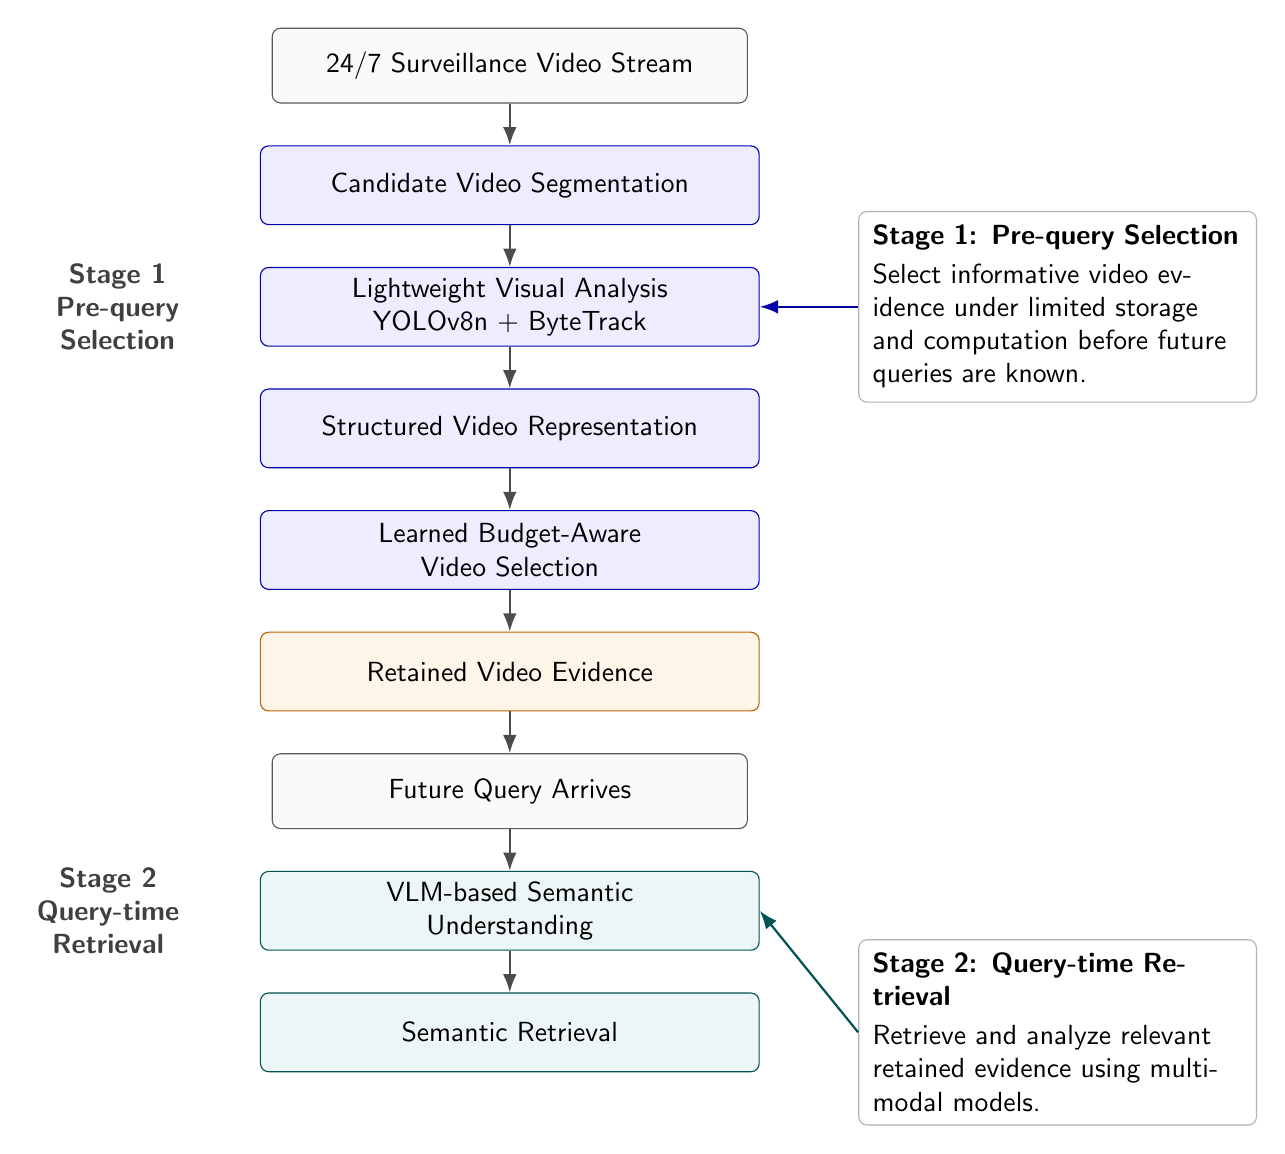
\begin{tikzpicture}[
  node distance=5.3mm,
  >=Latex,
  font=\sffamily,
  box/.style={
    rectangle,
    draw=black!65,
    rounded corners=3pt,
    align=center,
    minimum height=9.5mm,
    text width=5.8cm,
    fill=gray!4
  },
  stageone/.style={
    rectangle,
    draw=blue!70!black,
    rounded corners=3pt,
    align=center,
    minimum height=10mm,
    text width=6.1cm,
    fill=blue!7
  },
  stagetwo/.style={
    rectangle,
    draw=teal!65!black,
    rounded corners=3pt,
    align=center,
    minimum height=10mm,
    text width=6.1cm,
    fill=teal!7
  },
  boundary/.style={
    rectangle,
    draw=orange!75!black,
    rounded corners=3pt,
    align=center,
    minimum height=10mm,
    text width=6.1cm,
    fill=orange!9
  },
  note/.style={
    rectangle,
    draw=black!30,
    rounded corners=3pt,
    align=left,
    text width=4.7cm,
    inner sep=5pt,
    fill=white
  },
  stagelabel/.style={
    font=\sffamily\bfseries,
    align=center,
    text=black!75
  },
  arr/.style={->,thick,draw=black!70}
]

\node[box] (stream) {24/7 Surveillance Video Stream};
\node[stageone, below=of stream] (segment) {Candidate Video Segmentation};
\node[stageone, below=of segment] (analysis) {Lightweight Visual Analysis\\YOLOv8n + ByteTrack};
\node[stageone, below=of analysis] (structure) {Structured Video Representation};
\node[stageone, below=of structure] (selection) {Learned Budget-Aware\\Video Selection};
\node[boundary, below=of selection] (evidence) {Retained Video Evidence};
\node[box, below=of evidence] (query) {Future Query Arrives};
\node[stagetwo, below=of query] (understanding) {VLM-based Semantic\\Understanding};
\node[stagetwo, below=of understanding] (retrieval) {Semantic Retrieval};

\draw[arr] (stream) -- (segment);
\draw[arr] (segment) -- (analysis);
\draw[arr] (analysis) -- (structure);
\draw[arr] (structure) -- (selection);
\draw[arr] (selection) -- (evidence);
\draw[arr] (evidence) -- (query);
\draw[arr] (query) -- (understanding);
\draw[arr] (understanding) -- (retrieval);

\node[stagelabel, left=0.9cm of analysis] (stage1label) {Stage 1\\Pre-query\\Selection};
\node[stagelabel, left=0.9cm of understanding] (stage2label) {Stage 2\\Query-time\\Retrieval};

\node[note, right=1.25cm of analysis] (stage1note) {
  \textbf{Stage 1: Pre-query Selection}\\[2pt]
  Select informative video evidence under limited storage and computation before future queries are known.
};

\node[note, right=1.25cm of retrieval] (stage2note) {
  \textbf{Stage 2: Query-time Retrieval}\\[2pt]
  Retrieve and analyze relevant retained evidence using multimodal models.
};

\draw[arr, draw=blue!65!black] (stage1note.west) -- (analysis.east);
\draw[arr, draw=teal!65!black] (stage2note.west) -- (understanding.east);

\end{tikzpicture}
\end{document}
